\section{Appendix}

\crefalias{section}{appsec}
\newpage

\begin{landscape}
    \subsection{Literature on Trade Classification Using Machine Learning}
    \label{app:literature-ml-tc}
    \begin{table}[ht]
        \centering
        \caption[Literature on Trade Classification Using Machine Learning.]{Literature on trade classification using machine learning. Improvement is the out-of-sample performance over the best baselines if multiple baselines are reported. Data requirements may not be identical to these of classical rules.}
        \label{tab:literature-trade-classification-ml}
        \begin{tabular}{@{}p{3cm}p{3cm}lp{4cm}p{4cm}l@{}}
            \toprule
            Research                                                      & Data                              & Sample Period            & Method                                                                                                 & Baseline                                                     & Improvement              \\ \midrule
            \autocite[][15]{rosenthalModelingTradeDirection2012}          & \gls{NASDAQ}                      &                          & Logistic regression                                                                                    & \gls{EMO} rule, \gls{LR} rule,\newline and tick rule         & max. \SI{2.2}{\percent}  \\ \cmidrule{2-6}
                                                                          & \gls{NYSE}                        & 03/12/2004 -- 31/12/2004 & Logistic regression                                                                                    & \gls{EMO} rule, \gls{LR} rule,\newline and tick rule         & max. \SI{1.1}{\percent}  \\\cmidrule{1-6}
            \autocite[][489--494]{blazejewskiLocalNonParametricModel2005} & Australian Stock\newline Exchange & 11/11/2002 -- 27/08/2003 & $k$ nearest neighbour, \newline logistic regression,\newline trade continuation,\newline majority vote &                                                              &                          \\ \cmidrule{1-6}
            \autocite[][49--57]{ronenMachineLearningTrade2022}            & \gls{TRACE}                       & 01/07/2002 -- 31/12/2019 & Logistic regression, decision tree,\newline neural network, and random forests                         & \gls{LR} rule and tick rule,\newline and \gls{BVC} algorithm & max. \SI{13.3}{\percent} \\ \cmidrule{2-6}
                                                                          & \gls{NASDAQ}                      & 09/12/2013 -- 13/12/2013 & Logistic regression, decision tree,\newline neural network, and random forests                         & \gls{LR} rule, tick rule,\newline and \gls{BVC} algorithm    & max. \SI{3.3}{\percent}  \\ \bottomrule
        \end{tabular}
    \end{table}
\end{landscape}


\subsection{Power-Transforms of Features}
\label{app:power-transforms-of-features}

\begin{table}[ht]
    \centering
    \caption[Power-Transforms of Features]{Power-transforms of features. \lambda~specifies the exponent. Transformations estimated on \gls{ISE} training set.}
    \label{tab:power-transformerations}
    \begin{tabular}{lS}
        \toprule
        {Feature}        & {\lambda} \\
        \midrule
        strike price     & -0.082968 \\
        trade size       & -0.204893 \\
        trade price      & 0.060425  \\
        best bid         & 0.110299  \\
        best ask         & 0.056837  \\
        ask (ex)         & 0.049090  \\
        bid (ex)         & 0.113067  \\
        bid size (ex)    & 0.140284  \\
        ask size (ex)    & 0.029876  \\
        price lead (all) & 0.054975  \\
        price lag (all)  & 0.049097  \\
        price lead (ex)  & 0.053774  \\
        price lag (ex)   & 0.042910  \\
        day volume       & -0.116017 \\
        moneyness        & -0.109716 \\
        \bottomrule
    \end{tabular}
\end{table}

\subsection{Features and Transformations}
\label{app:feature-and-transformations}

\begin{table}[H]
    \centering
    \begin{threeparttable}
        \begin{tabular}{@{}lll@{}}
            \toprule
            Feature Name            & Definition                                                                                       & Transform              \\ \midrule
            trade price             & $P_{i, t}$                                                                                       & $\log$ + standardised  \\
            price lag (ex)          & $P_{i, t-1}^{\text{ex}}$\tnote{*}                                                                & $\log$ + standardised  \\
            price lag (all)         & $P_{i, t-1}^{\text{all}}$\tnote{*}                                                               & $\log$ + standardised  \\
            price change lag (ex)   & $P_{i, t-1}^{\text{ex}}/P_{i, t}^{\text{ex}}$\tnote{*}                                           & clipped + standardised \\
            price change lag (all)  & $P_{i, t-1}^{\text{all}}/P_{i, t}^{\text{all}}$\tnote{*}                                         & clipped + standardised \\
            price lead (ex)        & $P_{i, t+1}^{\text{ex}}$\tnote{*}                                                                & $\log$ + standardised  \\
            price lead (all)        & $P_{i, t+1}^{\text{all}}$\tnote{*}                                                               & $\log$ + standardised  \\
            price change lead (ex)  & $P_{i, t}^{\text{ex}}/P_{i, t+1}^{\text{ex}}$\tnote{*}                                           & clipped + standardised \\
            price change lead (all) & $P_{i, t}^{\text{all}}/P_{i, t+1}^{\text{all}}$\tnote{*}                                         & clipped + standardised \\
            bid (all)               & $B_{i, t}^{\text{all}}$                                                                          & $\log$ + standardised  \\
            bid (ex)                & $B_{i, t}^{\text{ex}}$                                                                           & $\log$ + standardised  \\
            ask (all)               & $A_{i, t}^{\text{all}}$                                                                          & $\log$ + standardised  \\
            ask (ex)                & $A_{i, t}^{\text{all}}$                                                                          & $\log$ + standardised  \\
            prox. to quotes (ex)    & $\left(P_{i, t}^{\text{ex}}- M_{i, t}^{\text{ex}}\right) / \tfrac{1}{2} S_{i, t}^{\text{ex}}$    & clipped + standardised \\
            prox. to quotes (all)   & $\left(P_{i, t}^{\text{all}}- M_{i, t}^{\text{all}}\right) / \tfrac{1}{2} S_{i, t}^{\text{all}}$ & clipped + standardised \\
            bid ask size ratio (ex) & $\tilde{B}_{i, t}^{\text{ex}}/\tilde{A}_{i, t}^{\text{ex}}$                                      & clipped + standardised \\
            bid size (ex)           & $\tilde{B}_{i, t}^{\text{ex}}$                                                                   & $\log$ + standardised  \\
            ask size (ex)           & $\tilde{A}_{i, t}^{\text{ex}}$                                                                   & $\log$ + standardised  \\
            rel. bid size (ex)      & $\tilde{B}_{i, t}^{\text{ex}}/\tilde{P}_{i, t}^{\text{ex}}$                                      & clipped + standardised \\
            rel. ask size (ex)      & $\tilde{A}_{i, t}^{\text{ex}}/\tilde{P}_{i, t}^{\text{ex}}$                                      & clipped + standardised \\
            trade size              & $\tilde{P}_{i, t}$                                                                               & $\log$ + standardised  \\
            strike price            &                                                                                                  & $\log$ + standardised  \\
            volume option series    &                                                                                                  & $\log$ + standardised  \\
            root                    &                                                                                                  & binarised              \\
            time to maturity        &                                                                                                  & standardised           \\
            moneyness               &                                                                                                  & standardised           \\
            option type             &                                                                                                  & binarised              \\
            issue type              &                                                                                                  & binarised              \\ \bottomrule
        \end{tabular}
        \begin{tablenotes}\footnotesize
            \item[*] Notation assumes, that the previous or next trade price is distinguishable.
        \end{tablenotes}
    \end{threeparttable}
    \caption[Overview of Features and Transformations]{Overview of Features and Transformations}
    \label{tab:features-transformations}
\end{table}

\newpage
\subsection{Autocorrelation of Features}
\label{app:autocorrelation-of-features}

\begin{figure}[ht]
    \centering
    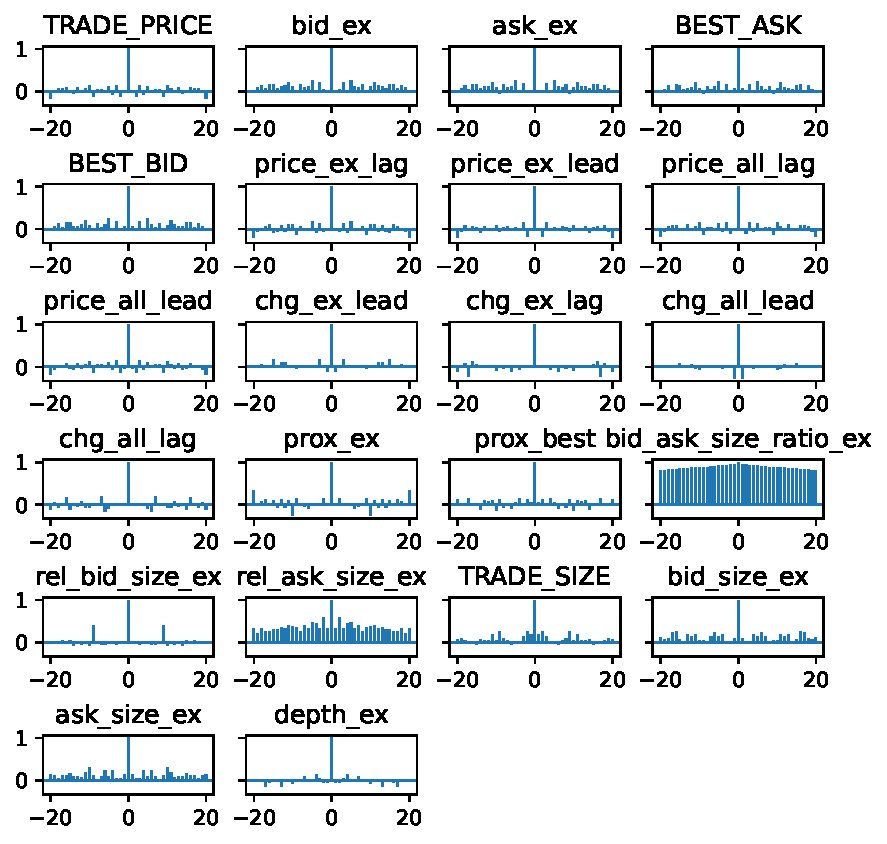
\includegraphics{auto-corr-features.pdf}
    \caption[Autocorrelation of Features]{Autocorrelation Features. Own work.}
    \label{fig:auto-correlation-features}
\end{figure}

\newpage
\subsection{Results of Supervised Models With Re-Training}
\label{app:results-of-supervised-models-with-re-training}

\begin{table}[ht]
    \centering
    \caption[Accuracies of Supervised Approaches With Re-Training On \glsentryshort{CBOE} and \glsentryshort{ISE}]{This table reports the accuracy of \glspl{GBRT} for different feature sets on the \gls{ISE} and \gls{CBOE} test set after re-training on \gls{ISE} training and validation set. The improvement is estimated as the absolute change in accuracy between the classifier and the benchmark. For feature set classical, $\operatorname{gsu}_{\mathrm{small}}$ is the benchmark and otherwise $\operatorname{gsu}_{\mathrm{large}}$.}
    \label{tab:results-supervised-retraining-ise-cboe}
    \begin{tabular}{@{}llSSSSSS@{}}
        \toprule
                   &            & \multicolumn{2}{c}{\gls{FS} Classical} & \multicolumn{2}{c}{\gls{FS} Classical-Size} & \multicolumn{2}{c}{\gls{FS} Option}                                      \\ \cmidrule(lr){3-4}\cmidrule(lr){5-6} \cmidrule(lr){7-8}
        Classifier & Data Set   & {Acc. in \%}                     & {+/-}                                 & {Acc. in \%}                  & {+/-}    & {Acc. in \%} & {+/-}    \\ \midrule
        \gls{GBRT} & \gls{ISE}  & 66.413827                        & 6.360000                              & 73.945544                     & 6.330000 & 76.162269    & 8.550000 \\
                   & \gls{CBOE} & 67.526839                        & 6.780000                              & 72.754664                     & 6.240000 & 75.125406    & 8.610000 \\ \bottomrule
    \end{tabular}
\end{table}
